\section{Experiments}

%In the experimental section, we first analyze the fitting capacity of the proposed neuron. We then performed experiments on both computer vision (CV) and natural language processing (NLP) tasks to compare the accuracy of the converted models. Then, we examine how different parameter settings affect the performance of the proposed method.

In this section, we evaluate the proposed PRIME framework on both computer vision (CV) and natural language processing (NLP) tasks. All the experiments are executed on a single NVIDIA A100 GPU with PyTorch 2.10.0 and CUDA 12.8. 
%\hwrevised{Note} that \textbf{\hwrevised{our method is training-free: all of the implementations are conducted on the weights of the corresponding pretrained ANN models.}}
%making it applicable to proprietary or frozen models where training pipeline access is unavailable.
%\hwrevised{\sout{We further examine how different parameter settings affect performance through ablation studies.}}
%All the experiments are executed on a single NVIDIA A100 GPU with PyTorch 2.10.0 and CUDA 12.8. 
%\hwrevised{Moreover, PRIME also supports other data %formats such as INT4 and FP8 besides FP16 operands as shown in Appendix~\ref{sec:fp8_int4}.}

\begin{table*}[t!]
  \centering
  \caption{Performance comparison of different methods on the ImageNet-1K dataset. ``Bits'' denotes the total number of bits transmitted across all timesteps (i.e., the cumulative bit-width of the spike over $T$ steps), reflecting the inter-layer data transmission cost during inference.}
  \label{tab:comparison}
  \resizebox{\textwidth}{!}{
  \begin{tabular}{llccccccc}
    \toprule
    Method & Arch. & Param.(M) & ANN Acc.(\%) & $T$ & Bits & SNN Acc.(\%) \\
    \midrule
    TS\cite{TS}
      & VGG-16         & 138.0    & 72.40 & 64           & 64          & 70.97~(-1.43) \\
    SNM\cite{SNM}
      & VGG-16         & 138.0    & 73.18 & 64           & 128         & 71.50~(-1.68) \\
    \cmidrule(lr){2-7}
    \multirow{2}{*}{QCFS\cite{QCFS}}
      & ResNet-34      & 21.8   & 74.32 & 64           & 64          & 72.35~(-1.97) \\
      & VGG-16         & 138.0    & 74.29 & 64           & 64          & 72.85~(-1.44) \\
    \cmidrule(lr){2-7}
    \multirow{2}{*}{SRP\cite{SRP}}
      & ResNet-34      & 21.8   & 74.32 & 64        & 64       & 68.61~(-5.71) \\
      & VGG-16         & 138.0    & 74.29 & 64        & 64       & 69.43~(-4.86) \\
    \cmidrule(lr){2-7}
    MST\cite{MST}
      & Swin-T         & 28.5   & 80.51 & 512     & 512    & 78.51~(-2.00) \\
    STA\cite{STA}
      & ViT-B/32       & 86.0     & 83.60 & 256      & 256     & 82.79~(-0.81) \\
    \cmidrule(lr){2-7}
    \multirow{3}{*}{SpikeZIP-TF\cite{spikeziptf}}
      & SViT-S-32 & 22.1  & 81.59 & 64           & 128         & 81.45~(-0.14) \\
      & SViT-B-32 & 86.6  & 82.83 & 64           & 128         & 82.71~(-0.12) \\
      & SViT-L-32 & 304.3 & 83.86 & 64           & 128         & 83.82~(-0.04) \\
    \cmidrule(lr){2-7}
    \multirow{2}{*}{ECMT\cite{ECMT}}
      & ViT-S/16       & 22.0     & 78.04 &10        & 40      & 77.07~(-0.97) \\
      & EVA-G          & 1074.0   & 89.62 &8         & 32      & 89.40~(-0.22) \\
    \cmidrule(lr){2-7}
    \makecell[l]{Adaptive fission\cite{adaptive}\\ + QCFS\cite{QCFS}}
      & ResNet-34      & 21.8   & 74.32 & 32           & 64          & 69.37~(-4.95) \\
    \cmidrule(lr){2-7}
    \multirow{4}{*}{DCGS\cite{dcgs}}
      & VGG-4/1        & 138.0    & 73.25 &  8         &  24      &  73.17~(-0.08) \\
      & ResNet34-4/1   & 21.8   & 76.42 & 8         &  24      &  76.04~(-0.38) \\
      & ViT-L-8/4      & 304.3  & 85.84 &  4         &  16       &  85.45~(-0.39) \\
      & EVA02-L-8/4    & 305.1  & 90.05 &  4         &  16       & 89.72~(-0.33) \\
    \midrule
    \multirow{10}{*}{\textbf{PRIME~(ours)}}
      & VGG-16         & 138.0    & 71.12 & \textbf{2} $(D{=}3)$  & \textbf{13}          & \textbf{71.08~(-0.04)} \\
      & ResNet-34      & 21.8   & 76.09 & \textbf{2} $(D{=}3)$  & \textbf{13}          & \textbf{76.13~(-0.00)} \\
      & ViT-S          & 22.1   & 78.04 & \textbf{2} $(D{=}3)$  & \textbf{13}          & \textbf{78.06~(-0.00)} \\
      & ViT-B          & 86.6   & 82.91 & \textbf{2} $(D{=}3)$  & \textbf{13}          & \textbf{82.87~(-0.04)} \\
      & ViT-L          & 304.3  & 84.88 & \textbf{2} $(D{=}3)$  & \textbf{13}          & \textbf{84.89~(-0.00)} \\
      & EVA02-T        & 5.8    & 80.62 & \textbf{2} $(D{=}3)$  & \textbf{13}          & \textbf{80.63~(-0.00)} \\
      & EVA02-S        & 22.1   & 85.73 & \textbf{2} $(D{=}3)$  & \textbf{13}          & \textbf{85.70~(-0.03)} \\
      & EVA02-B        & 87.1   & 88.26 & \textbf{2} $(D{=}3)$  & \textbf{13}          & \textbf{88.27~(-0.00)} \\
      & EVA02-L        & 305.1  & 89.63 & \textbf{2} $(D{=}3)$  & \textbf{13}          & \textbf{89.63~(-0.00)} \\
      & EVA02-G        & 1013.0   & 89.62 & \textbf{2} $(D{=}3)$  & \textbf{13}          & \textbf{89.58~(-0.04)} \\
    \bottomrule
  \end{tabular}
  }
\end{table*}

\subsection{Evaluation on Computer Vision Tasks}

For CV tasks, we validate the effectiveness of PRIME on the classic CNN and Transformer architectures, including VGG, ResNet, ViT, and EVA, evaluated on the ImageNet-1K~\cite{Imagenet} and CIFAR~\cite{cifar} (provided in Appendix~\ref{overall_cifars}, Figure~\ref{fig:cifar}) datasets. We follow the experimental settings of~\cite{ECMT}.

% ImageNet-1k Task
%\paragraph{ImageNet-1k Task}
% 3. Param.（M）加点表示省略
% 4. ACC. (%)
% 5. T那列CALIB和QCFS、TEBN有点抽象，有别的写法吗，如果没有，CALIB和QCFS可以加一个换行。
% T那列处理下之后整个表的字体应该就能放大了。

%The experimental results of the EVA and ViT series models on the ImageNet-1k dataset are shown in Table ~\ref{tab:comparison}:

The experimental results on ImageNet-1K are presented in Table~\ref{tab:comparison}. \hwrevised{The results show that} PRIME consistently achieves lower conversion error across both CNN and Transformer architectures. Compared with the classic baseline DCGS~(\cite{dcgs}), PRIME uses only two timesteps to achieve lower accuracy degradation on VGG and ResNet ($0.04\%$ vs. $0.08\%$, $0.00\%$ vs. $0.38\%$). It demonstrates more pronounced advantages on ViT and EVA architectures ($0.00\%$ vs. $0.39\%$, $0.00\%$ vs. $0.33\%$). In summary, PRIME is the closest to lossless ANN-to-SNN conversion among the existing frameworks in Table \ref{tab:comparison}, while further reducing the inter-layer bit-width during hardware deployment ($13$ bits vs. $16$ bits). (\hwrevised{For additional analysis, the full  results across all $(T, D)$ configurations are provided in Appendix~\ref{overall_imagenet} (Table~\ref{tab:appendix_imagenet}). )}


%暂时删除
%We first apply our method to the Transformer architecture and analyze the performance of the conversions. For ViT-B, our method achieves \textbf{82.87\%} at \(T=2\), outperforming STA~\cite{STA} (78.72\% at \(T=32\) and 82.79\% at \(T=256\)) and MST~\cite{MST} (77.88\% at \(T=128\)) with dramatically fewer timesteps. Against SpikeZIP-TF~\cite{spikeziptf}, which requires specialized SViT architectures and \(T=64\) to obtain 82.71\% in SViT-B, our method delivers a comparable accuracy (82.87\%) in standard ViT-B with only \(T=2\). Notably, on the large-scale EVA02-G (1,013M parameters), our method achieves \textbf{89.58\%} at \(T=2\), surpassing ECMT~\cite{ECMT} (89.40\% at \(T=8\)) and matching DCGS~\cite{dcgs} (89.72\% at \(T=4\)) while operating at lower latency and without architectural modifications.
%暂时删除
%For CNN-based conversion, our method also sets a new standard. On ResNet-34, it achieves \textbf{76.13\%} at \(T=2\), which is 4.01\% higher than QCFS~\cite{QCFS} (72.35\% at \(T=64\)) and 5.01\% higher than mmSE~\cite{MMSE} (71.12\% at \(T=64\)). On VGG-16, our method reaches 71.08\% at \(T=2\), outperforming TS~\cite{TS} (70.97\% at \(T=64\)) and SNM~\cite{SNM} (71.50\% at \(T=64\)) while using only \(1/32\) of the timesteps. These results highlight that our approach not only eliminates the latency bottleneck typical of CNN-to-SNN conversions, whereas it also improves accuracy over prior state-of-the-art.

% Finally, we emphasize the architectural generality of our method. It achieves consistent near-lossless conversion across a wide spectrum of models, from lightweight ViT-S (78.06\%) to the largest EVA02-G (89.58\%), and from VGG-16 to ResNet-34, with performance gaps never exceeding 0.05\%. In contrast, competing methods such as DCGS~\cite{dcgs} show larger discrepancies on smaller Transformer models (e.g., EVA02-T drops from 80.63\% ANN to 66.32\% at \(T=2\)), underscoring the robustness of our design.

% Taken together, these results establish our method as a highly efficient, scalable, and architecture-agnostic solution for low-latency SNN deployment. To the best of our knowledge, this is the first conversion framework that consistently achieves >85\% ImageNet accuracy with as few as two timesteps, bridging the gap between ANN and SNN performance without sacrificing efficiency.
%%%dcgs的部分减少一点

% \paragraph{CIFAR-10 and CIFAR-100 Task}

% % \begin{wraptable}{r}{0.62\textwidth}
% %   \centering
% %   \vspace{-1em}  % 微调垂直对齐
% %   \caption{Classification Accuracy on CIFAR-10 and CIFAR-100 (\%)}
% %   \begin{tabular}{lccccc}
% %     \toprule
% %     Dataset & \(D\) & \(T\!=\!1\) & \(T\!=\!2\) & \(T\!=\!3\) & ANN \\
% %     \midrule
% %     \multirow{3}{*}{CIFAR-10}
% %     & 1 & 70.27 & 97.97 & 98.40 & 98.42 \\
% %     & 2 & 96.57 & 98.41 & 98.40 & — \\
% %     & 3 & 98.05 & 98.37 & 98.43 & — \\
% %     \midrule
% %     \multirow{3}{*}{CIFAR-100}
% %     & 1 & 36.70 & 87.95 & 89.46 & 89.81 \\
% %     & 2 & 83.07 & 89.40 & 89.82 & — \\
% %     & 3 & 88.59 & 89.82 & 89.75 & — \\
% %     \bottomrule
% %   \end{tabular}
% %   \label{tab:cifar_all}
% % \end{wraptable}

% \begin{figure}[ht!]
%     \centering
%     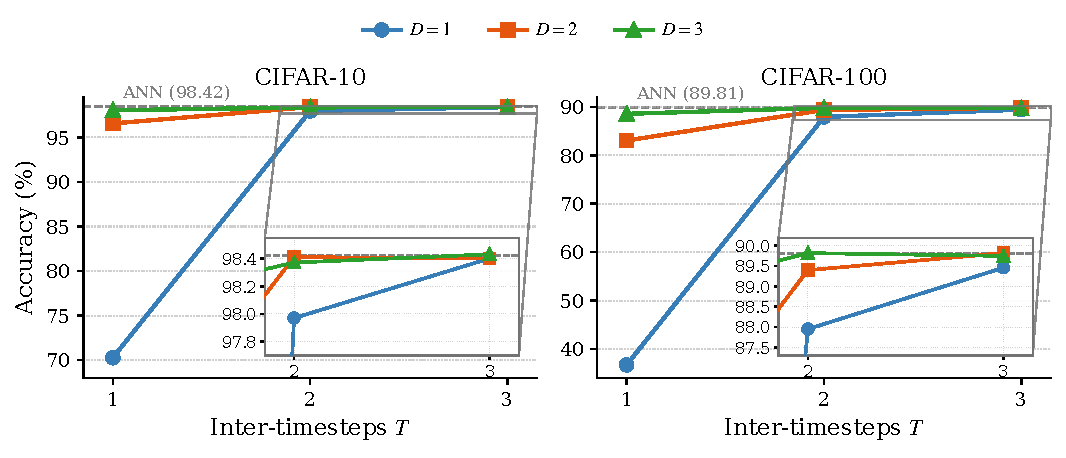
\includegraphics[width=0.7\linewidth]{Figs_new/cifar_accuracy.pdf}
%     \caption{Enter Caption}
%     \label{fig:calc}
% \end{figure}

% We evaluate the converted ViT-S model in CIFAR tasks under different combinations of parameters and report the post-conversion accuracy in table~\ref{tab:cifar_all}
% .In this experiment, we evaluate our method on CIFAR-10 and CIFAR-100 under varying network depths \(D\) and timesteps \(T\). Following common practices in SNN conversion, we adopt the same architectural configurations as the ANN counterparts without additional modifications. The results are presented in Table~\ref{tab:cifar_all}. For CIFAR-10, with \(D=1\), our method achieves \textbf{98.40\%} accuracy at \(T=3\), closely matching the ANN baseline (98.42\%) while requiring only 3 timesteps. Remarkably, even at \(T=2\), the accuracy reaches 97.97\%, with a negligible drop of 0.45\%. For CIFAR-100, our method attains \textbf{89.46\%} at \(T=3\) and 87.95\% at \(T=2\), again approaching the baseline of the ANN of 89.81\%.

% We further observe that deeper networks enable faster convergence. With \(D=3\), the SNN on CIFAR-10 already reaches 98.05\% at \(T=1\) and saturates at 98.37\% for \(T=3\), effectively matching the ANN. Similarly, on CIFAR-100, \(D=3\) yields 88.59\% at \(T=1\) and 89.82\% at \(T=2\), narrowing the gap to within 0.06\% of the ANN. These results demonstrate that our method achieves almost lossless conversion with as few as \(T=2\) timesteps, and deeper architectures further reduce the required latency. 

% % \begin{table}[htbp]
% %   \centering
% %   \caption{Classification Accuracy on CIFAR-10 and CIFAR-100 (\%)}
% %   \begin{tabular}{lccccc}
% %     \toprule
% %     Dataset & \(D\) & \(T\!=\!1\) & \(T\!=\!2\) & \(T\!=\!3\) & ANN \\
% %     \midrule
% %     \multirow{3}{*}{CIFAR-10}
% %     & 1 & 70.27 & 97.97 & 98.40 & 98.42 \\
% %     & 2 & 96.57 & 98.41 & 98.40 & — \\
% %     & 3 & 98.05 & 98.37 & 98.43 & — \\
% %     \midrule
% %     \multirow{3}{*}{CIFAR-100}
% %     & 1 & 36.70 & 87.95 & 89.46 & 89.81 \\
% %     & 2 & 83.07 & 89.40 & 89.82 & — \\
% %     & 3 & 88.59 & 89.82 & 89.75 & — \\
% %     \bottomrule
% %   \end{tabular}
% %   \label{tab:cifar_all}
% % \end{table}

\subsection{Evaluation on Natural Language Tasks}

For NLP tasks, we conduct the evaluations on Qwen, Llama, and OPT series models~\cite{qwen3,llama2,zhang2022opt}. The evaluations \hwrevised{perform} on the \hwrevised{primary NLP} benchmarks, including MMLU, PIQA, ARC-C, ARC-E, Winogrande, and Hellaswag~\cite{mmlu,piqa,wiqa, arc}. The evaluation process is implemented based on the work of~\cite{eval-harness}. We evaluate our method on the common sense reasoning tasks by converting LLAMA2-7b and LLAMA2-13b models with ultra-low latency ($T=2$). Following common practices in SNN conversion, we apply the same architectural configurations for our method. 
The results are presented in Table~\ref{tab:commonsense} and indicate that \hwrevised{ our method maintains an accuracy loss of less than 0.3$\%$ on the aforementioned NLP benchmarks.}
To the best of our knowledge, this is the first ANN-to-SNN conversion framework that consistently attains $<$0.3\% accuracy degradation on common-sense reasoning benchmarks, with only 2 timesteps. 
More results under different settings and datasets are shown in Appendix~\ref{overall_mmlu} (Figure~\ref{fig:mmlu}), Appendix~\ref{overall_llama} (Table~\ref{tab:appendix_llama}), and Appendix~\ref{overall_qwen3} (Table~\ref{tab:appendix_qwen3_mmlu}).
Notably, for other bit precision, our proposed method can also be applied effectively. 
The conversion results for FP8- and INT4-quantized LLMs are provided in Appendix~\ref{sec:fp8_int4}.


% \paragraph{OPT Model Results.}
% We also evaluate PRIME on the OPT model family~\cite{zhang2022opt} to enable direct comparison with FAS~\cite{fas} and LAS~\cite{las}, which report results exclusively on OPT. Due to space constraints, detailed OPT results are provided in Appendix~\ref{sec:opt_results}. In summary, PRIME achieves comparable or superior accuracy to LAS (T=16, 64 bits) while operating at T=2 with only 13 bits, representing a $5\times$ reduction in latency and a $4.9\times$ reduction in bit-transmission cost.

%\paragraph{Comparison of Common Tasks for NLP to SNN Conversion}
%Tasks such as PIQA, ARC-C, ARC-E, Winogrande, and Hellaswag are frequently adopted in NLP-to-SNN conversion works. We also conduct evaluations on these tasks and the results are shown in Table~\ref{tab:commonsense}.

\begin{table*}[htbp]
  \centering
  \caption{Performance Comparison on Common Sense Reasoning Tasks (\%). ``Bits'' denotes the total bits transmitted across all timesteps, reflecting the data transmission cost during inference.}
  \label{tab:commonsense}
  \resizebox{\textwidth}{!}{
  \begin{tabular}{llcccccccccc}
    \toprule
    Method & Model & Spike & $T$ & Bits & PIQA & ARC-c\_n & ARC-e\_n & Winog. & HellS.\_n \\
    \midrule

    \multirow{2}{*}{LLAMA}
      & LLAMA2-7b  & $\times$ & N/A          & 16 & 78.45 & 45.73 & 74.87 & 69.38 & 76.28 \\
      & LLAMA2-13b & $\times$ & N/A          & 16 & 80.52 & 48.89 & 76.56 & 72.22 & 79.71 \\

    \multirow{2}{*}{SpikeLLM\cite{spikellm}}
      & LLAMA2-7b  & $\checkmark$ & 2        & 32 & 65.67 & 28.41 & 41.88 & 52.80 & 49.87 \\
      & LLAMA2-13b & $\checkmark$ & 2        & 32 & 67.68 & 30.38 & 44.53 & 57.22 & 58.02 \\

    FAS\cite{fas}
      & OPT-7B     & $\checkmark$ & 16       & 32 & 73.23 & ---   & 64.73 & 60.38 & ---   \\

    \multirow{3}{*}{LAS\cite{las}}
      & OPT-7B     & $\checkmark$ & 16       & 64 & 76.22 & ---   & 65.95 & 65.75 & ---   \\
      & OPT-13B    & $\checkmark$ & 16       & 64 & 76.28 & ---   & 67.38 & 65.51 & ---   \\
      & OPT-66B    & $\checkmark$ & 16       & 64 & 78.67 & ---   & 71.25 & 68.27 & ---   \\

    \cmidrule{1-10}

    \multirow{2}{*}{PRIME~(ours)}
      & LLAMA2-7b  & $\checkmark$ & \textbf{2 $(D{=}3)$} & \textbf{13} & \textbf{78.67} & \textbf{45.65} & \textbf{74.75} & \textbf{69.06} & \textbf{76.18} \\
      & LLAMA2-13b & $\checkmark$ & \textbf{2 $(D{=}3)$} & \textbf{13} & \textbf{80.58} & \textbf{49.15} & \textbf{76.47} & \textbf{72.14} & \textbf{79.69} \\

    \bottomrule
  \end{tabular}
  }
\end{table*}
% \begin{wraptable}{r}{0.55\textwidth}
%   \centering
%   \vspace{-1em}
%   \caption{MMLU Performance Comparison}
%   \label{tab:mmlu}
%   \begin{tabular}{ccc}
%     \toprule
%     Model & ANN & Converted(T=2,D=3) \\
%     \midrule
%     llama2-7b        & 45.75 & 45.95 \\
%     llama2-13b       & 55.13 & 55.31 \\
%     qwen3-0.6b-base  & 52.41 & 52.60 \\
%     qwen3-1.7b-base  & 62.61 & 62.26 \\
%     qwen3-4b-base    & 72.90 & 72.92 \\
%     qwen3-8b-base    & 76.85 & 76.90 \\
%     qwen3-14b-base   & 80.47 & 80.49 \\
%     \bottomrule
%   \end{tabular}
% \end{wraptable}
% QKV的Spike怎么实现不关


% Ablation study moved to Appendix~\ref{sec:ablation_expdim}.
\subsection{Ablation Study}

By default, we adopt the full FP16 exponent bit-width (5 bits) to set the threshold range, which preserves conversion accuracy. To evaluate the trade-off between efficiency and accuracy, we reduce the exponent bit-width to 4 and report the results in Table~\ref{tab:ablation2}. Across all $(T, D)$ configurations, the accuracy drop is marginal, while the number of active thresholds and the inter-layer bit-transmission cost is substantially reduced. This confirms that the proposed threshold-range optimization offers a practical knob for resource-constrained deployment with negligible performance sacrifice.
\hwrevised{More} ablation results on  the query spiking strategy in Transformer attention are provided in Appendix~\ref{sec:query_ablation}.
%(Table~\ref{tab:query}).

\begin{table*}[htbp]
  \centering
  \scriptsize  
  \caption{Ablation study on lightweight threshold-range optimization via exponent-bit 
  width reduction (\texttt{width=4}) on ImageNet-1K, evaluated across different 
  $(T, D)$ settings. \texttt{Default} refers to the full fp16 exponent-bit width 
  , with spike conversion applied to $k$ and $v$ only in Transformer 
  blocks.}
  \label{tab:ablation2}
  \resizebox{\textwidth}{!}{
  \begin{tabular}{cccccccccc}
    \toprule
    \multirow{2}{*}{Model} & \multirow{2}{*}{ANN} & \multirow{2}{*}{D} 
    & \multicolumn{3}{c}{Default} 
    & \multicolumn{3}{c}{Exponent-bit width $= 4$} \\
    \cmidrule(lr){4-6} \cmidrule(lr){7-9}
    & & & $T=1$ & $T=2$ & $T=3$ & $T=1$ & $T=2$ & $T=3$ \\
    \midrule
    \multirow{3}{*}{ViT-S (patch16\_224)} 
    & \multirow{3}{*}{78.04} 
    & 1 & 48.20 & 76.27 & 77.80 & 55.26 & 76.29 & 77.47 \\
    & & 2 & 73.78 & 77.94 & 78.03 & 73.94 & 77.66 & 77.65 \\
    & & 3 & 77.01 & 78.06 & 78.03 & 76.92 & 77.66 & 77.65 \\
    \midrule
    \multirow{3}{*}{ViT-B (patch16\_224)}
    & \multirow{3}{*}{82.91} 
    & 1 & 74.00 & 82.21 & 82.74 & 75.80 & 81.30 & 81.77 \\
    & & 2 & 80.89 & 82.77 & 82.89 & 80.30 & 81.74 & 81.88 \\
    & & 3 & 82.41 & 82.87 & 82.91 & 81.38 & 81.87 & 81.87 \\
    \midrule
    \multirow{3}{*}{ViT-L (patch16\_224)} 
    & \multirow{3}{*}{84.88} 
    & 1 & 80.89 & 84.46 & 84.79 & 81.14 & 83.81 & 84.31 \\
    & & 2 & 84.03 & 84.80 & 84.89 & 83.25 & 84.31 & 84.32 \\
    & & 3 & 84.45 & 84.89 & 84.88 & 84.01 & 84.30 & 84.30 \\
    \bottomrule
  \end{tabular}
  }
\end{table*}




% In the default setting, we directly use the exponent bits of fp16 as thresholds, 
% which improves conversion accuracy and eliminates the need for additional threshold 
% computation during ANN-to-SNN conversion, thereby  improving the conversion 
% efficiency. However, the default fp16 exponent bit width corresponds to a relatively 
% large number of thresholds. In deployment scenarios sensitive to hardware resources or 
% bit-transmission cost beween layers, 
% we propose a lightweight threshold-range optimization scheme that 
% reduces active exponent bits 
% and decreasing the bit-transmission cost beween layers. 
% We set the bit-width to \texttt{exp\_dim=4} and the results 
% are presented in Table~\ref{tab:ablation2}, 
% with
% only a marginal accuracy drop across different $(T, D)$ 
% settings, while substantially reducing the threshold count.

% \symrevising{In the default setting, we directly adopt the exponent bit-width of FP16 as the threshold bit-width, which preserves conversion accuracy without requiring additional threshold computation. However, the full FP16 exponent bit-width corresponds to a relatively large number of thresholds. For deployment scenarios sensitive to hardware resources or inter-layer transmission cost, we propose a lightweight threshold-range optimization scheme that reduces the number of active exponent bits, thereby lowering the inter-layer bit-transmission cost. We set the exponent bit-width to \texttt{Exponent-bit width=4}, and the results are presented in Table~\ref{tab:ablation2}. Only a marginal accuracy drop is observed across different $(T, D)$ settings, while the threshold count is substantially reduced.}